\documentclass[12pt,letterpaper]{article}
\usepackage{amsmath}
\usepackage[utf8]{inputenc}
\usepackage{graphicx}
\usepackage{wrapfig}

\title{\textbf{Existencia de la economia dual en Colombia}}
\author{Augusto Rico}
\date{\today}

\graphicspath{{Fig/}}

\newcommand*{\captionsource}[2]{%
    \textbf{\\Tomado:} #2%
  }%


\begin{document}
\maketitle
\section{Introduccion}

\begin{flushleft}   


El siguiente articuló esta enfocado en comprobar empíricamente la existencia de una economía dual en Colombia tal como plantea Lewis(1954).
Esta hipótesis se basa en la consideración por parte del FMI(2020) de Colombia como una economía en vía de Desarrollo, por ende si esto es cierto 
y basándonos en la tesis de W. Arthur Lewis Colombia debe tener también las características de una economía Dual.\\
~\\
Las economías en vía de desarrollo tal como plantea Lewis(1954) están caracterizadas por la coexistencia de dos tipos de economía, la moderna caracterizada
por altos niveles relativos de productividad, ya que son intensivas en bienes de capital, y la economía tradicional caracterizada por bajos niveles de productividad, 
debido a la no existencia de bienes de capital en este sector, lo que implica bajos salarios para los trabajadores.\\
~\\
En Colombia este hecho se puede ver reflejado principalmente en las diferencias económicas entre las ciudades principales y las zonas rurales, que como se expondrá
las ciudades principales están caracterizadas por tener sectores modernos e industriales con altos niveles relativos de ingresos y bienestar, y las zonas rurales
apartadas del centro caracterizadas por la escasez de bienes de capital y un fuerte sector rural con baja productividad sostenido por uso intensivo de mano de obra con salarios de subsistencia.\\
~\\
En el trabajo se evaluara la existencia de una economía dual en Colombia, mediante indicadores de ingresos, calidad de vida, capacidad productiva para comprender si
existe efectivamente las dos economías en Colombia, para esto se evaluara los datos según divisiones administrativas, ya que aunque puedan coexistir estas dos economías por ejemplo en Bogotá
se tiene datos insuficientes para poder evaluarlo a una escala inferior.\\

\end{flushleft}

\section{Contexto Geografico e Historico}

\begin{flushleft}

Los habitantes de las distintas regiones del país han estado históricamente aislados por la complicada geografía nacional. Esto ha generado una clara desigualdad en el desarrollo nacional, 
el cual ha estado marcado por bonanzas de materias primas, principalmente café y petróleo, que logro mejorar las condiciones económicas y productivas de las zonas donde eran explotados estos recursos, y el periodo de
Sustitución de importaciones donde se inició con el proceso de industrializacion, pero focalizado únicamente en las ciudades principales generando claras diferencias entre la división centro-periferia. (Hahn \& Mesiel, 2018) \\
~\\
Dada la naturaleza centralista de Colombia y tal como afirman Junguito \& Rincon (2004) con un aumento del gasto público que paso en la primera mitad del siglo XX del 5 a cerca del 10\% del PIB en 1990 impulso
principalmente el desempeño económico de Bogotá, que adicionalmente con el proceso de sustitución de importaciones le genero un mayor impulso a la desigualdad entre centro y periferia debido a que
mientras las ciudades principales eran beneficiadas gracias a la industrializacion las regiones periféricas que el gobierno central no se interesó en industrializar sufrían el aumento en los costes asociados de producción lo que reducía su capacidad de inversión
y por ende una incapacidad de lograr aumentar su productividad.\\
~\\

\end{flushleft}

\newpage

\section{Desigualdad de ingresos}

\begin{flushleft}

La característica principal de un mercado con economía dual es la abrupta diferencia entre los empleados del sector moderno y tradicional, ya que esto denota
la expansión heterogénea del capitalismo en una zona, hecho que se ve reflejado en Colombia tal como planteaba Furtado(1959) con una dominación-dependencia en las relaciones centro-periferia nacionales
donde los altos ingresos se encuentran concentrados en las ciudades principales del país con procesos capitalistas equiparables a países desarrollados mientras 
se tiene zonas periféricas con procesos pseudo-feudales intensivos en mano de obra por el desinterés del centro para desarrollar estas economías.\\ 
~\\
\begin{figure}[h!]
    \centering
    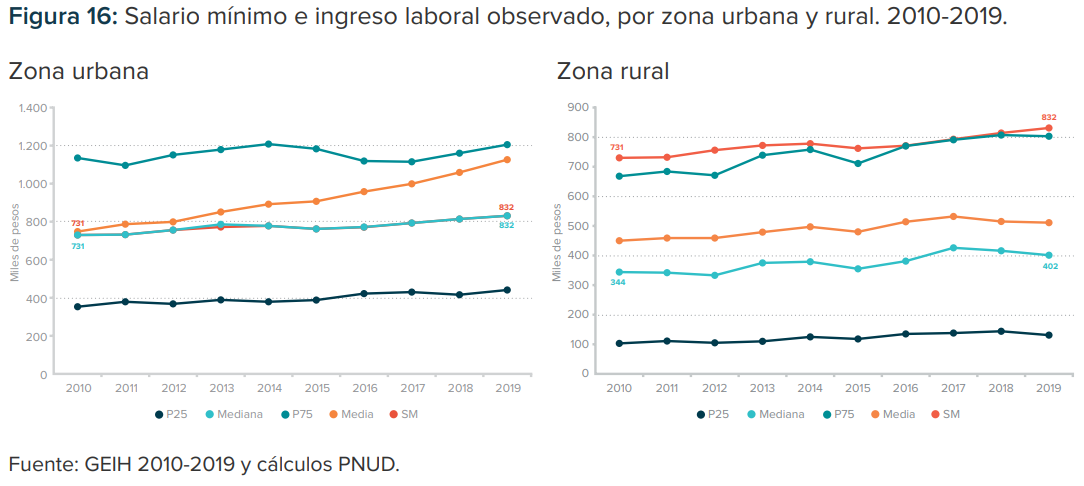
\includegraphics[width=\linewidth]{ingcentro-perisferia.png}
    \captionsource{Caption}{Mision de Empleo (2021)}
\end{figure}

Tal como se observa en las gráficas en Colombia existe una clara economía dual medida mediante los ingresos laborales, mientras en las zonas urbanas el salario mínimo se ajusta a la mediana del salario,
en las zonas rurales en cambio el salario mínimo no es siquiera superado por tres cuartas partes de los trabajadores rurales lo que evidencia una clara desigualdad en los ingresos entre estas dos economías.\\
~\\
\begin{figure}[h!]
    \centering
    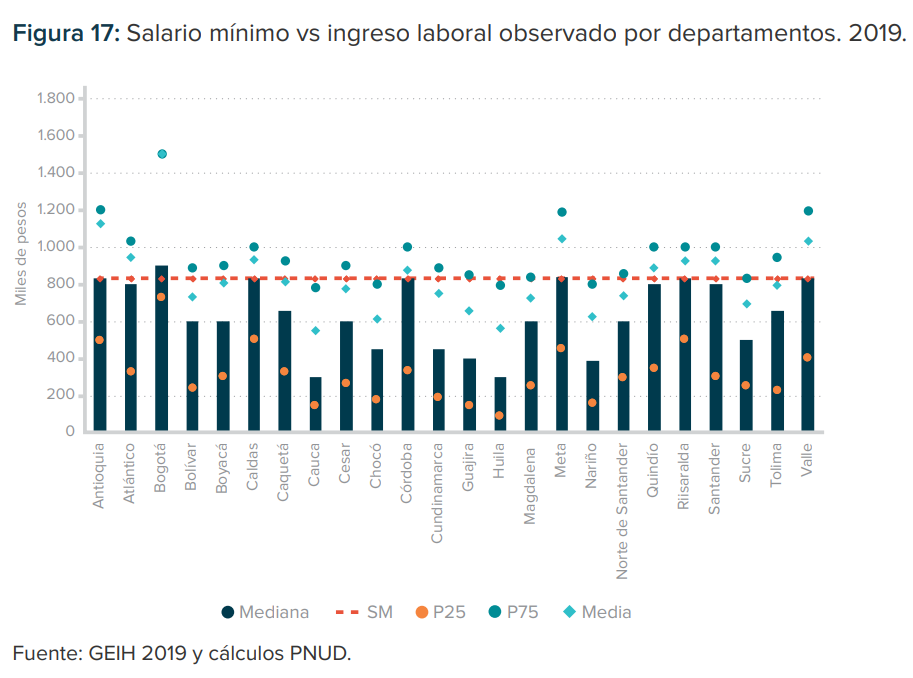
\includegraphics[scale=0.5]{ingdepto.png}
    \captionsource{Caption}{Mision de Empleo (2021)}
\end{figure}

Si este mismo análisis es realizado mediante la comparación de ingresos en departamentos se obtiene mejores evidencias de la existencia de una economía dual en Colombia enmarcada en una fuerte dependencia
centro-periferia donde la única zona que logra que su mediana de salario supere el salario mínimo es Bogotá, la capital, y se le acercan zonas económicamente centrales tales como Atlántico, Antioquia, y Valle del Cauca u otras zonas que en algún punto
han experimentado bonanzas tales como la zona cafetera o petrolera.\\
\end{flushleft}

\newpage

\section{Flujos Migratorios Internos}



\begin{flushleft}


Una de las principales características del merado laboral colombiano es la profunda heterogeneidad regional, aun cuando las normas laborales son nacionales, 
donde una de las principales diferencias es la diferencia de productividad y sus tasas de informalidad en consiguiente. (Arango \& Florez, 2017)\\
~\\

debido a la existencia del salario mínimo en Colombia, no se puede plantear una expansión del capitalismo en los mercados precapitalistas de Colombia,
debido a que el salario mínimo no se ajusta a los niveles de productividad de estas zonas por lo que las empresas capitalistas prefieren primero establecerse en 
las zonas de mayor productividad posible para poder obtener los mayores rendimientos. Por lo que a diferencia de la teoría de las economías duales donde 
se argumenta que las empresas capitalistas logran contratar de forma ilimitada a salario de subsistencia, el cual se puede asumir como la mediana del salario, no es posible en Colombia 
y por ende lo que se genera en cambio son procesos de migración internos de zonas precapitalistas con bajos niveles de productividad y un salario mínimo relativamente alto a zonas capitalistas con un ajuste entre la productividad y el salario mínimo.\\

~\\
Por lo cual la absorción de la mano de obra tradicional por parte del sector moderno en Colombia se puede entender mediante los flujos migratorios internos
provenientes de departamentos periféricos hacia las economías centrales. Esto sin ignorar el contexto de violencia que pueda tambien existir en los desplazamientos.\\
~\\

\newpage

\begin{figure}[h!]
    \centering
    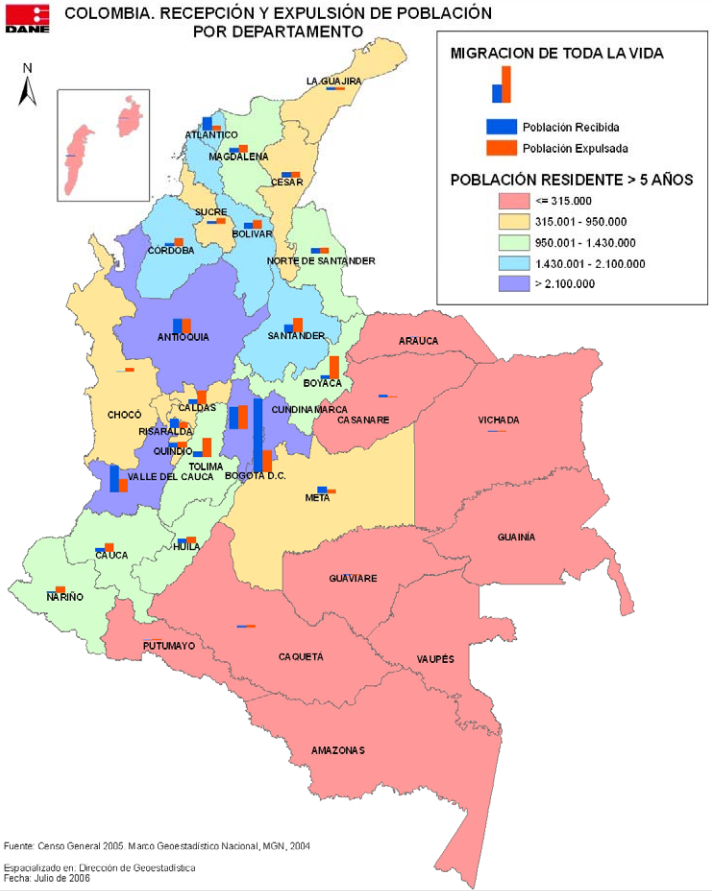
\includegraphics[scale=0.4]{flujos.png}
    \captionsource{Caption}{Dane, Censo 2005}
\end{figure}

En concordancia con la teoría de la economía dual y lo expuesto anteriormente se puede observar que el mayor receptor neto de flujos migratorios internos
 son Bogotá y otras zonas centrales como Atlántico y Valle del Cauca, mientras que zonas que presentaban bajos niveles de ingresos tales como Cauca, Nariño o Boyacá son expulsores de población, 
 por lo que se puede comprender que en Colombia está existiendo una absorción perfecta por parte del sector moderno tal como plantea la teoría.



\end{flushleft}

\newpage

\section{Conclusiones}

\begin{flushleft}
    \begin{itemize}
        \item Es posible concluir que tal como plantea Lewis(1954) Colombia se puede considerar una economía dual con ciertas particularidades
        debido a la coexistencia del sector tradicional y moderno en el país.
        \item La economía dual colombiana está caracterizada por una relación de dominancia por parte de las economías céntricas sobre las zonas periféricas, 
        lo que ha generado una profunda heterogeneidad entre las zonas modernas y tradicionales.
        \item Debido a la existencia de normas laborales nacionales como el salario mínimo la absorción por parte del sector moderno del sector tradicional está caracterizada por migraciones internas.
    \end{itemize}


\end{flushleft}

\newpage

\section{Bibliografía}

\begin{flushleft}
    \begin{itemize}
        \item Arango, L. E., \& Flórez, L. A. (2018). Informalidad laboral y elementos para un salario mínimo diferencial por regiones en Colombia. Borradores de Economía; No. 1023.
        \item DANE, Censo General. (2005).
        \item Fernández, M., González, S., \& Rosero, A. Misión de Empleo 2020-2021.
        \item Lewis, W. A. (1954). Economic development with unlimited supplies of labour.
        \item Junguito, R., \& Rincón, H. (2004). La política fiscal en el siglo XX en Colombia. Borradores de economía, 318.
        \item Ortega, M. A. (2018). Conectando mercados: vías rurales y producción agrícola en el contexto de una economía dual (Connecting markets: rural roads and agricultural production in a dual economy). Documento CEDE, (2018-44).
        \item Hahn, L., Meisel, A. (2018). La desigualdad económica entre las regiones de Colombia, 1926-2016. Cuadernos de Historia Económica; No. 47.
    \end{itemize}
\end{flushleft}

\end{document}